% This file was created with tikzplotlib v0.9.12.
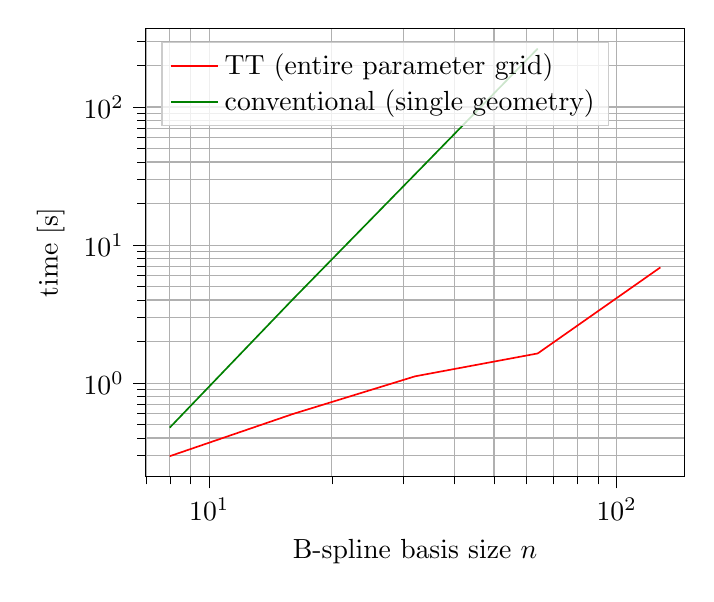
\begin{tikzpicture}

\begin{axis}[
legend cell align={left},
legend style={
  fill opacity=0.8,
  draw opacity=1,
  text opacity=1,
  at={(0.03,0.97)},
  anchor=north west,
  draw=white!80!black
},
log basis x={10},
log basis y={10},
tick align=outside,
tick pos=left,
unbounded coords=jump,
x grid style={white!69.0196078431373!black},
xlabel={B-spline basis size \(\displaystyle n\)},
xmajorgrids,
xmin=6.96440450636899, xmax=147.03338943962,
xminorgrids,
xmode=log,
xtick style={color=black},
y grid style={white!69.0196078431373!black},
ylabel={time [s]},
ymajorgrids,
ymin=0.210445817165706, ymax=372.507358532735,
yminorgrids,
ymode=log,
ytick style={color=black}
]
\addplot [semithick, red]
table {%
8 0.295649
16 0.596063
32 1.120147
64 1.640698
128 6.892718
};
\addlegendentry{TT (entire parameter grid)}
\addplot [semithick, green!50!black]
table {%
8 0.476336
16 4.019093
32 32.580096
64 265.15434
128 nan
};
\addlegendentry{conventional (single geometry)}
\end{axis}

\end{tikzpicture}
